%   % !TEX root = ../../VIII,3_Rahmen-TeX_8-1.tex
%
%
%   Band VIII, 3 N.~??S01.09
%   Signatur/Tex-Datei: LH_35_09_23_021-022
%   RK-Nr. 41208 /9
%   \ref{dcc_07}
%   Überschrift: De corporum concursus scheda septima
%   Modul: Mechanik / Stoß ()
%   Datierung: Januar 1678
%   WZ: (Bl. 22) LEd-WZ 803017 = RK-WZ 1264 (insgesamt: eins)
%   SZ: (keins)
%   Bilddateien (PDF):
%                     LH_35_09_23_021-022_d1 ((ex: lh0350923_021r-d1)); 
%                     LH_35_09_23_021-022_d2 ((ex: lh0350923_021v-d1)); 
%                     LH_35_09_23_021-022_d3 ((ex: lh0350923_022r-d1)) 
%                     (insgesamt: drei)
%   Verzeichniseinträge: vollständig
%   \textls{} statt \textso{} (Ausnahme: Personenverzeichnis)
%
%
\selectlanguage{ngerman}%
\frenchspacing%
%
\begin{ledgroupsized}[r]{120mm}%
\footnotesize%
\pstart%
\noindent%
\textbf{Überlieferung:}%
\pend%
\end{ledgroupsized}%
\begin{ledgroupsized}[r]{114mm}%
\footnotesize%
\pstart%
\parindent -6mm%
\makebox[6mm][l]{\textit{L}}%
Konzept:
LH XXXV~9, 23 Bl.~21\textendash22.
Ein Bogen 2\textsuperscript{o};
ein Wasserzeichen auf Bl.~22.
Vier vollbeschriebene Seiten.
Randbemerkungen zum Teil \textit{post reformationem} verfasst (siehe die editorische Vorbemerkung, S.~\refpassage{dcc_Vorbemerkung_reform-1}{dcc_Vorbemerkung_reform-2}).
\pend%
\end{ledgroupsized}%
%
\begin{ledgroupsized}[r]{114mm}%
\footnotesize%
\pstart%
\parindent -6mm%
\makebox[6mm][l]{\textit{E}}%
\textsc{Fichant} 1994, S.~145\textendash151\cite{01056}
(mit kommentierter französischer Übersetzung, S.~278\textendash302).
\pend%
\end{ledgroupsized}%
%
\selectlanguage{latin}%
\frenchspacing%
%
%
\vspace{8mm}%
\count\Bfootins=1000%
\count\Afootins=1200%
\count\Cfootins=1000
\normalsize%
\pstart%
\noindent%
%
\lbrack21~r\textsuperscript{o}\rbrack%   %  %  %  %  Blatt 21r 
\hspace{45mm}
Scheda septima%
\protect\index{Sachverzeichnis}{scheda}%
\hspace{35mm}
Januar. 1678%
\pend%
%
\pstart%
\noindent%
\centering%
de concursu corporum%
\protect\index{Sachverzeichnis}{concursus corporum}%
\pend%
\vspace{0.5em}%
%
\pstart%
\noindent%
\edtext{%
Quamquam superiora
certis positionibus factis,
ut
%
\edtext{si corpora dura%
\protect\index{Sachverzeichnis}{corpus durum}
et homogenea%
\protect\index{Sachverzeichnis}{corpus homogeneum}
et percussionis capacia%
\protect\index{Sachverzeichnis}{corpus percussionis capax}
intelligantur,}{%
\lemma{si}\Bfootnote{%
\textit{(1)}~corpus aliquod
\textit{(2)}~corpora dura et homogenea et
\textit{(a)}~nihil
\textit{(b)}~percussionis capacia intelligantur,%
~\textit{L}}}
%
satis recte procedere arbitrer;
juvat tamen rem omnem
nova velut luce affulgente%
\protect\index{Sachverzeichnis}{lux affulgens}
de integro
\edlabel{LH_35_09_23_021-022_021r1}%
ordiri:%
%
}{%
\lemma{\textit{Am Rand:}}\Afootnote{%
Imo in illis error%
\protect\index{Sachverzeichnis}{error}
etiam ex hypothesi homogeneitatis%
\protect\index{Sachverzeichnis}{hypothesis homogeneitatis}%
\lbrack;\rbrack\
nam servanda summa
possibilis%
\textsuperscript{[a]}
similitudo effectus cum causa%
\protect\index{Sachverzeichnis}{similitudo effectus cum causa}%
\protect\index{Sachverzeichnis}{causa et effectus}%
\protect\index{Sachverzeichnis}{effectus et causa}%
\lbrack,\rbrack\
et quidem ex capitibus diversis%
\lbrack,\rbrack\
calculum mutat,%
\protect\index{Sachverzeichnis}{calculus}
ut%
\textsuperscript{[b]}
et ostendimus
tam ex percussione%
\protect\index{Sachverzeichnis}{percussio}
sub%
\textsuperscript{[c]}
finem schedae quintae%
\protect\index{Sachverzeichnis}{scheda}%
\lbrack,\rbrack\
quam etiam alias%
\textsuperscript{[d]}
ex conservatione virium%
\protect\index{Sachverzeichnis}{conservatio virium}
quae non ex celeritatibus
sed celeritatum quadratis fiunt,%
\protect\index{Sachverzeichnis}{quadratum celeritatis}
non posse priores ratiocinationes%
\protect\index{Sachverzeichnis}{ratiocinatio}
schedae 1, 2 etc. stare%
\protect\index{Sachverzeichnis}{scheda}
quoad lineas rectas%
\protect\index{Sachverzeichnis}{linea recta}
ibi%
\textsuperscript{[e]}
assignatas.%
\newline\vspace{-0.4em}%
\newline%
{\footnotesize%
%
\textsuperscript{[a]}~%
possibilis
\textit{erg.~L}
\quad
%
\textsuperscript{[b]}~%
ut
\textit{(1)}~supra
\textit{(2)}~et ostendimus tam ex percussione 
\textit{(a)}~quam ex
\textit{(b)}~sub finem \lbrack...\rbrack\ quam etiam
\textbar~alias \textit{erg.}~%
\textbar\ ex conservatione virium%
~\textit{L}
\quad
%
\textsuperscript{[c]}~%
sub \lbrack...\rbrack\ quintae:
N.~\ref{dcc_05}, %??S01\textsubscript{6}, 
S.~\refpassage{LH_35_09_23_012v_sbchj-1}{LH_35_09_23_012v_sbchj-2}.
\quad
%
\textsuperscript{[d]}~%
alias:
N.~\ref{dcc_08}, %??S01\textsubscript{10}, 
S.~\pageref{LH_37_05_086v_vaikea}\,ff.
\quad
%
\textsuperscript{[e]}~%
ibi:
N.~\ref{dcc_01}, %??S01\textsubscript{1},
S.~\refpassage{LH_35_09_23_002r_probaturrecta_mxyz-1}{LH_35_09_23_002r_probaturrecta_mxyz-2};
N.~\ref{dcc_02-1}, %??S01\textsubscript{2},
S.~\refpassage{LH_35_09_23_003v_recta_lje-1}{LH_35_09_23_003v_recta_lje-2};
vgl. auch
N.~\ref{dcc_03}, %??S01\textsubscript{4},
S.~\refpassage{LH_35_09_23_007r_estrecta_jmgt-1}{LH_35_09_23_007r_estrecta_jmgt-2}.\vspace{-3mm}%
}}}
%
\edtext{}{%
{\xxref{LH_35_09_23_021-022_021r1}{LH_35_09_23_021-022_021r2}}%
{\lemma{ordiri:}\Bfootnote{%
\textit{(1)}~Caus
\textit{(2)}~\textls{Effectus}%
~\textit{L}}}}%
%
\pend%
%
\pstart%
\textls{Effectus}%
\edlabel{LH_35_09_23_021-022_021r2}%
\textls{ integer assimilatur causae plenae }%
quoad ejus fieri potest.%
\protect\index{Sachverzeichnis}{effectus integer}%
\protect\index{Sachverzeichnis}{causa plena}%
\protect\index{Sachverzeichnis}{similitudo effectus cum causa}
Nam effectus integer tantum causae plenae mutatio est quaedam,%
\protect\index{Sachverzeichnis}{mutatio causae plenae}
et quidem quam
%
%\edtext{\lbrack tam\rbrack}{%
%\lemma{quam}\Bfootnote{%
%\textit{L~ändert Hrsg.}}}
%
\edtext{minima fieri}{%
\lemma{minima}\Bfootnote{\hspace{-0,5mm}%
\textbar~quam \textit{streicht Hrsg.}~\textbar\ fieri%
~\textit{L}}}
%
potest.
Ex. gr. status Mundi praesens%
\protect\index{Sachverzeichnis}{status mundi praesens}%
\protect\index{Sachverzeichnis}{mundus}
quam minime differet a sua causa integra,%
\protect\index{Sachverzeichnis}{causa integra}
scil. statu praecedenti.%
\protect\index{Sachverzeichnis}{status mundi praecedens}
Nimirum Effectus%
\protect\index{Sachverzeichnis}{effectus et causa}
et causa%
\protect\index{Sachverzeichnis}{causa et effectus}
tantum formali quodam peculiari differunt,
in summa conveniunt.
Quemadmodum
%
\edtext{si ex triangulo \textit{ABC}%
\protect\index{Sachverzeichnis}{triangulum}
fiat quadratum \textit{BDCE},%
\protect\index{Sachverzeichnis}{quadratum}}{%
\lemma{si}\Bfootnote{%
\textit{(1)}~corpus aliquod
\textit{(2)}~ex triangulo \lbrack...\rbrack\ quadratum \textit{BDCE},%
~\textit{L}}}
%%
%\begin{wrapfigure}{l}{0.20\textwidth}
%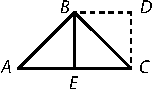
\includegraphics[width=0.16\textwidth]{gesamttex/edit_VIII,3/images/LH_35_09_23_021-022_d1.pdf}\\
%%\rule[0pt]{10mm}{0pt}
%\lbrack\textit{Fig.~1}\rbrack\
%\end{wrapfigure}
%
%{\raisebox{-1.05em}{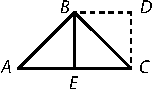
\includegraphics[width=0.148\textwidth]{gesamttex/edit_VIII,3/images/LH_35_09_23_021-022_d1.pdf}}}
%\lbrack\textit{Fig.~1}\rbrack\
%
non \makebox[1.0\textwidth][s]{differunt
%
\edtext{magnitudine.
Machinae%
\protect\index{Sachverzeichnis}{machina}%
}{%
\lemma{magnitudine}\Bfootnote{%
\textit{(1)}~, si con
\textit{(2)}~. Machinae%
~\textit{L}}}
%
alicujus status%
\protect\index{Sachverzeichnis}{status machinae praesens}
%
\edtext{\lbrack praesens\rbrack}{%
\lemma{praecedens}\Bfootnote{%
\textit{L~ändert Hrsg. nach~E, S.~145}\cite{01056}}}
%
differt a praecedente%
\protect\index{Sachverzeichnis}{status machinae praecedens}%
\lbrack,\rbrack\
situ}
\pend
\newpage
%  \newpage% 
 % \vspace{1.5em}%	% Diagramm Fig.~1
  \centerline{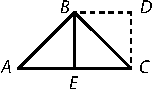
\includegraphics[width=0.22\textwidth]{gesamttex/edit_VIII,3/images/LH_35_09_23_021-022_d1.pdf}}%
  \vspace*{0.5em}
  \centerline{\lbrack\textit{Fig.~1}\rbrack}%
%  \label{LH_35_09_23_021r_Fig.~1}%
  \vspace{1.5em}%
%  \newpage%
%
\pstart
\noindent
%
\edtext{quidem potentiarum,%
\protect\index{Sachverzeichnis}{situs potentiae}%
\protect\index{Sachverzeichnis}{potentia machinae}
sed non}{%
\lemma{quidem}\Bfootnote{%
\textit{(1)}~non vero
\textit{(2)}~potentiarum, sed non%
~\textit{L}}}
%
earum summa.%
\protect\index{Sachverzeichnis}{summa potentiae}%
\protect\index{Sachverzeichnis}{potentia machinae}
Effectus integer%
\protect\index{Sachverzeichnis}{effectus integer}
oritur ex causa integra;%
\protect\index{Sachverzeichnis}{causa integra}
et
%
\edtext{conceptus effectus%
\protect\index{Sachverzeichnis}{conceptus effectus}%
}{%
\lemma{conceptus}\Bfootnote{%
\textit{(1)}~causae integrae
\textit{(2)}~effectus%
~\textit{L}}}
%
oritur ex conceptu causae,%
\protect\index{Sachverzeichnis}{conceptus causae}
quatenus simul necessitatem mutationis involvit.%
\protect\index{Sachverzeichnis}{necessitas mutationis}
Mutatio autem semper quam minima intelligitur.%
\protect\index{Sachverzeichnis}{mutatio inter causam et effectum}%
\protect\index{Sachverzeichnis}{mutatio quam minima}
\pend%
\pstart%
\edtext{Hinc\textls{ Effectus}}{%
\lemma{Hinc}\Bfootnote{%
\textit{(1)}~vis
\textit{(2)}~\textls{Effectus}%
~\textit{L}}}%
%
\textls{ integer aequipollet causae plenae,}
seu eandem habet potentiam.%
\protect\index{Sachverzeichnis}{effectus integer}%
\protect\index{Sachverzeichnis}{causa plena}%
\protect\index{Sachverzeichnis}{aequipollentia causae et effectus}%
\protect\index{Sachverzeichnis}{potentia causae}%
\protect\index{Sachverzeichnis}{potentia effectus}
Est corollarium praecedentis,%
\protect\index{Sachverzeichnis}{corollarium}
quia nulla potest esse necessitas mutandi potentiam,%
\protect\index{Sachverzeichnis}{necessitas mutandi potentiam}
etsi sit necessitas mutandi situm.%
\protect\index{Sachverzeichnis}{necessitas mutandi situm}
Nota\lbrack:\rbrack\
in rigore metaphysico%
\protect\index{Sachverzeichnis}{rigor metaphysicus}
Mundi%
\protect\index{Sachverzeichnis}{mundus}
vel alterius Machinae%
\protect\index{Sachverzeichnis}{machina}
status%
\protect\index{Sachverzeichnis}{status mundi}%
\protect\index{Sachverzeichnis}{status machinae}
praecedens non est causa sequentis,%
\protect\index{Sachverzeichnis}{status praecedens causa sequentis}
sed DEus,%
\protect\index{Sachverzeichnis}{Deus causa status sequentis}
quanquam status praecedens sequentis 
%
\edtext{\lbrack et\rbrack}{%
\lemma{et}\Bfootnote{\textit{erg. Hrsg.}}}
%
secuturi certum indicium.%
\protect\index{Sachverzeichnis}{indicium}%
\protect\index{Sachverzeichnis}{status praesens indicium sequentis}
Sed nos
%
\edtext{hic \lbrack physice\rbrack}{%
\lemma{hic}\Bfootnote{%
\textit{(1)}~pr
\textit{(2)}~in causae
\textit{(3)}~\textbar~physicae \textit{ändert Hrsg.}~\textbar%
~\textit{L}}}
%
loquimur,
neque inde error oriri potest,%
\protect\index{Sachverzeichnis}{error}
eo ipso quia indicium certum est.%
\protect\index{Sachverzeichnis}{indicium}
\pend%%
%
\pstart%
Eadem semper manet quantitas virium%
\protect\index{Sachverzeichnis}{quantitas virium}
in eadem Machina%
\protect\index{Sachverzeichnis}{machina}
seu corporum quotcunque
in actione aut passione constitutorum
aggregato.%
\protect\index{Sachverzeichnis}{aggregatum corporum}%
\protect\index{Sachverzeichnis}{actio corporis}%
\protect\index{Sachverzeichnis}{passio corporis}
Excluditur autem corpus
%
\edtext{externum%
\protect\index{Sachverzeichnis}{corpus externum}
vel}{%
\lemma{externum}\Bfootnote{%
\textit{(1)}~in quale null
\textit{(2)}~vel%
~\textit{L}}}
%
certe non consideratur.
\pend%%
%
\pstart%
Eadem est semper quantitas virium in mundo,%
\protect\index{Sachverzeichnis}{quantitas virium in mundo}%
\protect\index{Sachverzeichnis}{vis in mundo}
quia totus Mundus est una Machina.%
\protect\index{Sachverzeichnis}{mundus ut machina}
\pend%%
%
\pstart%
Hinc eadem semper est in Mundo quantitas Motus.%
\protect\index{Sachverzeichnis}{quantitas motus in mundo}
%
\edtext{}{%
\lemma{\textit{Am Ende des Absatzes:}}\Afootnote{%
Dubium de quantitate motus,%
\protect\index{Sachverzeichnis}{quantitas motus in mundo}
verum de quantitate virium.%
\protect\index{Sachverzeichnis}{quantitas virium in mundo}%
}}
%
\pend%
%
\pstart%
Corpus aliquod semel quiescens
aut in aliquam tendens plagam%
\lbrack,\rbrack\
semper quiescet%
\protect\index{Sachverzeichnis}{corpus quiescens}
aut in eam plagam eadem celeritate tendet;%
\protect\index{Sachverzeichnis}{corpus in plagam tendens}%
\protect\index{Sachverzeichnis}{plaga}
%
\edtext{patet quia}{%
\lemma{patet}\Bfootnote{%
\textit{(1)}~ex
\textit{(2)}~quia%
~\textit{L}}}
%
sequens status%
\protect\index{Sachverzeichnis}{status sequens effectus praecedentis}
%
\edtext{est effectus}{%
\lemma{est}\Bfootnote{%
\textit{(1)}~causa
\textit{(2)}~effectus%
~\textit{L}}}
%
praecedentis et
%
\edtext{nihil impedit}{%
\lemma{nihil}\Bfootnote{%
\textit{(1)}~refert
\textit{(2)}~impedit%
~\textit{L}}}
%
unum alteri assimilari.%
\protect\index{Sachverzeichnis}{assimilatio status praecedentis et sequentis}%
\protect\index{Sachverzeichnis}{assimilatio causae et effectus}
Si corpus incurrat in aliud aequale quiescens%
\protect\index{Sachverzeichnis}{incursus corporis in aequale quiescens}%
\protect\index{Sachverzeichnis}{corpus incurrens}%
\protect\index{Sachverzeichnis}{corpus quiescens}%
\protect\index{Sachverzeichnis}{corpora aequalia}
%
\edtext{durum%
\protect\index{Sachverzeichnis}{corpus durum}
vel satis Elasticum,%
\protect\index{Sachverzeichnis}{corpus elasticum}%
}{%
\lemma{durum}\Bfootnote{%
\hspace{-0,5mm}vel satis Elasticum
\textit{erg.~L}}}
%
ipsum in ejus loco quiescet,
corpus autem excipiens%
\protect\index{Sachverzeichnis}{corpus excipiens}
eadem qua incurrens venerat celeritate,%
\protect\index{Sachverzeichnis}{celeritas incursus}
in eandem plagam progredietur.%
\protect\index{Sachverzeichnis}{progressus in eandem plagam}%
\protect\index{Sachverzeichnis}{plaga}
Sequitur manifeste ex
%
\edtext{praecedenti.
Ita enim}{%
\lemma{praecedenti.}\Bfootnote{%
\textit{(1)}~Neque enim
\textit{(2)}~Ita enim%
~\textit{L}}}
%
maxime effectus causae,%
\protect\index{Sachverzeichnis}{causa et effectus}%
\protect\index{Sachverzeichnis}{effectus et causa}
vel status sequens praecedenti assimilatur.%
\protect\index{Sachverzeichnis}{assimilatio causae et effectus}
Nam perinde
quasi nihil occurrisset,
evenit%,
\lbrack;\rbrack\
%
\edtext{nam etsi corpus incurrens quieverit,}{%
\lemma{nam}\Bfootnote{%
\textit{(1)}~loco quiescenti
\textit{(2)}~etsi corpus incurrens quieverit,%
~\textit{L}}}
%
tamen excipiens vicarium aequale%
\protect\index{Sachverzeichnis}{corpus excipiens vicarium}%
\protect\index{Sachverzeichnis}{corpus excipiens aequale}
ipsi successit,
ita ergo in eandem
%
\edtext{\lbrack plagam\rbrack%
\protect\index{Sachverzeichnis}{plaga}%
}{%
\lemma{plagam}\Bfootnote{%
\textit{erg. Hrsg. nach~E, S.~146}\cite{01056}}}
%
eadem quantitas motus,%
\protect\index{Sachverzeichnis}{quantitas motus eadem}
id est vis pariter%
\protect\index{Sachverzeichnis}{vis manens}
et directio manet.%
\protect\index{Sachverzeichnis}{directio manens}
Usque adeo,
ut si corpora duo essent similia,%
\protect\index{Sachverzeichnis}{corpora similia}
ne discerni quidem omnino posset
status praecedens a%
\protect\index{Sachverzeichnis}{status praecedens}
%
\edtext{sequenti.%
\protect\index{Sachverzeichnis}{status sequens}
Quod}{%
\lemma{sequenti.}\Bfootnote{%
\textit{(1)}~Nam
\textit{(2)}~Quod%
~\textit{L}}}
%
si dissimilia sint
%
\edtext{discerni poterit}{%
\lemma{discerni}\Bfootnote{%
\textit{(1)}~poterunt
\textit{(2)}~poterit%
~\textit{L}}}
%
effectus a causa,%
\protect\index{Sachverzeichnis}{effectus a causa discernibilis}%
\protect\index{Sachverzeichnis}{causa et effectus}%
\protect\index{Sachverzeichnis}{effectus et causa}
sed non ratione virium earumque directionis;
et vero mutatio figurae%
\protect\index{Sachverzeichnis}{mutatio figurae}%
\protect\index{Sachverzeichnis}{figura mutata}
ex hoc quidem capite sequi non potest
cum corpus durum%
\protect\index{Sachverzeichnis}{corpus durum}
vel se restituens supponatur.%
\protect\index{Sachverzeichnis}{corpus se restituens}
Universaliter si duo corpora aequalia in eadem recta concurrant,%
\protect\index{Sachverzeichnis}{corpora concurrentia aequalia}
sive sibi occurrant,
sive assequantur,
sive excipiant,
semper fiet permutatio celeritatum%
\protect\index{Sachverzeichnis}{permutatio celeritatum}
et directionum.%
\protect\index{Sachverzeichnis}{permutatio directionum}
Ita enim quam maxime effectus assimilabitur causae.%
\protect\index{Sachverzeichnis}{assimilatio causae et effectus}%
\protect\index{Sachverzeichnis}{causa et effectus}%
\protect\index{Sachverzeichnis}{effectus et causa}
\pend%
%
\pstart%
Idem etiam ex hoc solo
quod corpus aequale incurrens in aequale quiescens%
\protect\index{Sachverzeichnis}{corpus incurrens in aequale quiescens}%
\protect\index{Sachverzeichnis}{corpus quiescens}%
\protect\index{Sachverzeichnis}{corpora aequalia}
ipsum abripit,%
\protect\index{Sachverzeichnis}{corpus abreptum}%
\protect\index{Sachverzeichnis}{abreptio}
demonstrari potest.
Nam si incurrat in aequale antecedens,%
\protect\index{Sachverzeichnis}{corpus incurrens in aequale antecedens}
tunc incurret
%
\edtext{ut}{%
\lemma{ut}\Bfootnote{%
\textit{erg.~L}}}
%
in quiescens%
\protect\index{Sachverzeichnis}{corpus incurrens in aequale quiescens}%
\protect\index{Sachverzeichnis}{corpus quiescens}%
\protect\index{Sachverzeichnis}{corpora aequalia}
differentia celeritatum,%
\protect\index{Sachverzeichnis}{differentia celeritatum}
et ambo simul ferentur
celeritate communi%
\protect\index{Sachverzeichnis}{celeritas communis}
seu
%
\edtext{minoris.%
\protect\index{Sachverzeichnis}{corpus minus}%
}{%
\lemma{minoris}\Cfootnote{%
Hier und im Folgenden (bis S.~\refpassage{LH_35_09_23_021v_dtwp}{LH_35_09_23_021v_dtwp}) sind \textit{minus} und \textit{majus} (\textit{corpus}) wohl hinsichtlich der Bewegungsgröße zu verstehen, denn hinsichtlich der Masse sind die zwei Körper als gleich gesetzt worden.
Siehe hierzu \textsc{Fichant} 1994, S.~147.\cite{01056}}}
%
Ergo dabit minori
differentiam celeritatum;
ipsumque minus%
\protect\index{Sachverzeichnis}{corpus minus}
praeterea et sua,
id est communi
feretur,
communis autem cum differentia%
\protect\index{Sachverzeichnis}{differentia celeritatum}
facit majorem;%
\protect\index{Sachverzeichnis}{celeritas major}
incurrens%
\protect\index{Sachverzeichnis}{corpus incurrens}
vero retinet sibi communem%
\protect\index{Sachverzeichnis}{celeritas communis}
tantum seu minorem.%
\protect\index{Sachverzeichnis}{celeritas minor}
Ergo si corpora
%
\edtext{aequalia%
\protect\index{Sachverzeichnis}{corpora aequalia assequentia}%
}{%
\lemma{aequalia}\Bfootnote{%
\textit{erg.~L}}}
%
se
%
\edtext{assequantur,
permutantur celeritates et directiones,%
\protect\index{Sachverzeichnis}{permutatio celeritatum}%
\protect\index{Sachverzeichnis}{permutatio directionum}
id est
directiones manent\protect\index{Sachverzeichnis}{directio manens}%
}{%
\lemma{assequantur,}\Bfootnote{%
\textit{(1)}~permutatur
\textit{(2)}~permutantur celeritates
\textit{(a)}~manent
\textit{(b)}~et directiones,
\textit{(aa)}~vel q
\textit{(bb)}~id est directiones manent%
~\textit{L}}}
%
quia eaedem.
\edlabel{LH_35_09_23_021r/v_jaezgvk-1}%
Denique
si duo corpora aequalia sibi occurrant,%
\protect\index{Sachverzeichnis}{corpora aequalia sibi occurrentia}
%
\edtext{tunc%
\lbrack,\rbrack\
si}{%
\lemma{tunc}\Bfootnote{\hspace{-0,5mm}%
\textit{(1)}~quatenus
\textit{(2)}~\textbar~cum \textit{streicht Hrsg.}~\textbar\
\textit{(3)}~\textlangle unam\textrangle\
\textit{(4)}~si%
~\textit{L}}}
%
aequali celeritate%
\lbrack,\rbrack\
necessario ambo redibunt%
\protect\index{Sachverzeichnis}{celeritas reditionis aequalis}
qua venere via,
%
\lbrack21~v\textsuperscript{o}\rbrack\  %  %  %  %  Blatt 21v
%
\edtext{nempe permutabuntur}{%
\lemma{nempe}\Bfootnote{%
\textit{(1)}~permutantur
\textit{(2)}~permutabuntur%
~\textit{L}}}
%
celeritates%
\protect\index{Sachverzeichnis}{permutatio celeritatum}
et directiones,%
\protect\index{Sachverzeichnis}{permutatio directionum}
id est manebunt celeritates%
\protect\index{Sachverzeichnis}{celeritas manens eadem}
(quippe eaedem),
permutabuntur directiones.%
\protect\index{Sachverzeichnis}{directio permutata}%
\edlabel{LH_35_09_23_021r/v_jaezgvk-2}
Si%
\edlabel{LH_35_09_23_021v_conflictus-1}
%
\edtext{vero corpora aequalia occurrant%
\protect\index{Sachverzeichnis}{corpora aequalia occurrentia}
sibi inaequali celeritate,%
\protect\index{Sachverzeichnis}{occursus inaequali celeritate}%
\protect\index{Sachverzeichnis}{celeritas inaequalis}%
}{%
\lemma{vero}\Bfootnote{%
\textit{(1)}~inaequalia sint
\textit{(2)}~corpora aequalia % occurrant sibi 
\lbrack...\rbrack\ inaequali celeritate,%
~\textit{L}}}
%
\edtext{tunc corpus velocius}{%
\lemma{tunc}\Bfootnote{%
\textit{(1)}~corpus minus et majus quatenus
\textit{(2)}~corpus velocius%
~\textit{L}}}
%
intelligatur ferri duplici celeritate,
nempe celeritate minoris
%
\edtext{et differentia celeritatum%
\protect\index{Sachverzeichnis}{differentia celeritatum}%
}{%
\lemma{et}\Bfootnote{%
\textit{(1)}~celeritate
\textit{(2)}~differentia celeritatum%
~\textit{L}}}
%
seu excessu%
\protect\index{Sachverzeichnis}{excessus celeritatis}%
\lbrack;\rbrack\
quatenus fertur communi%
\protect\index{Sachverzeichnis}{celeritas communis}
cum minore,%
\protect\index{Sachverzeichnis}{celeritas minor}
eatenus concurrentia duo corpora%
\protect\index{Sachverzeichnis}{corpora concurrentia}
conabuntur regredi%
\protect\index{Sachverzeichnis}{conatus regrediendi}
ea qua venerunt via,%
\protect\index{Sachverzeichnis}{via concursus}
%
\edtext{per priora,}{%
\lemma{per priora}\Cfootnote{%
Vgl. S.~\refpassage{LH_35_09_23_021r/v_jaezgvk-1}{LH_35_09_23_021r/v_jaezgvk-2}.%
}}
%
id est minus%
\protect\index{Sachverzeichnis}{corpus minus}
celeritate sua,%
\protect\index{Sachverzeichnis}{celeritas corporis minoris}
et majus celeritate ejusdem.
Verum cum majus adhuc habeat celeritatem excessus,%
\protect\index{Sachverzeichnis}{celeritas excessus}
jam quaestio est%
\protect\index{Sachverzeichnis}{quaestio}
an in majore%
\protect\index{Sachverzeichnis}{corpus majus}
confligere inter se%
\protect\index{Sachverzeichnis}{conatus confligentes}
ac a se invicem destrui,%
\protect\index{Sachverzeichnis}{conatus destructus}
id est in quantum destruuntur
in contrarium transferri debeant hi duo conatus,%
\protect\index{Sachverzeichnis}{conatus translatus in contrarium}
%
\edtext{sed hoc
%
\edtext{\lbrack positum\rbrack}{%
\lemma{posito}\Bfootnote{%
\textit{L~ändert Hrsg.}}}
%
contra ratiocinationem%
\protect\index{Sachverzeichnis}{ratiocinatio}
nostram eveniret;}{%
\lemma{\textit{Am Rand:}}\Afootnote{%
Imo nulla hic absurditas,%
\protect\index{Sachverzeichnis}{absurditas}
ut statim patebit.\textsuperscript{[a]}
\newline\vspace{-0.4em}%
\newline%
{\footnotesize%
\textsuperscript{[a]}~statimt patebit:
Vgl. S.~\refpassage{LH_35_09_23_021vstatimpatebit-1}{LH_35_09_23_021vstatimpatebit-2}.\vspace{-3mm}%
}}}
%
nimirum posito
excessum%
\protect\index{Sachverzeichnis}{excessus celeritatis}
esse ipsa minori%
\protect\index{Sachverzeichnis}{celeritas minor}
majorem,
%
\edtext{tunc minus%
\protect\index{Sachverzeichnis}{corpus minus}%
}{%
\lemma{tunc}\Bfootnote{%
\textit{(1)}~fere
\textit{(2)}~minus%
~\textit{L}}}
%
dupla celeritate
%
et recurreret,%
\protect\index{Sachverzeichnis}{corpus recurrens}
%\edtext{}{%
%\lemma{et}\Bfootnote{%
%\textit{(1)}~praetere
%\textit{(2)}~recurreret%
%~\textit{L}}}
%
et majus%
\protect\index{Sachverzeichnis}{corpus majus}
retineret excessum%
\protect\index{Sachverzeichnis}{excessus celeritatis}
excessus supra
%
\edtext{minorem.%
\protect\index{Sachverzeichnis}{celeritas minor}%
\edlabel{LH_35_09_23_021v_dtwp}
Itaque}{%
\lemma{minorem.}\Bfootnote{%
\textit{(1)}~Sed
\textit{(2)}~Itaque%
~\textit{L}}}
%
hoc modo labefactantur etiam
%
\edtext{quaedam meae superiores ratiocinationes,%
\protect\index{Sachverzeichnis}{ratiocinatio labefacta}%
}{%
\lemma{quaedam \lbrack...\rbrack\ ratiocinationes}\Cfootnote{%
Wohl N.~\ref{dcc_04}, %??S01\textsubscript{5} 
S.~\refpassage{LH_35_09_23_009rv_conflictus-1}{LH_35_09_23_009rv_conflictus-2}.%
}}
%
\edtext{\lbrack quas\rbrack}{%
\lemma{quae}\Bfootnote{%
\textit{L~ändert Hrsg.}}}
%
vel ideo
%
\edtext{subsistere posse dubitabam,}{%
\lemma{subsistere}\Bfootnote{%
\textit{(1)}~non poterant
\textit{(2)}~posse dubitabam,%
~\textit{L}}}
%
quod in
%
\edtext{illis sequi videtur}{%
\lemma{illis}\Bfootnote{%
\textit{(1)}~sequitur
\textit{(2)}~sequi videtur%
~\textit{L}}}
%
mutatio per%
\protect\index{Sachverzeichnis}{mutatio per saltum}
%
\edtext{saltum.%
\protect\index{Sachverzeichnis}{saltus}
Res accurate consideranda}{%
\lemma{saltum}\Bfootnote{%
\textit{(1)}~, nimirum si majus est
\textit{(a)}~fortius
\textit{(b)}~fortior est excessus
\textit{(2)}~. Res accurate consideranda%
~\textit{L}}}%
\lbrack,\rbrack\
est enim maximi momenti\lbrack:\rbrack\
\pend%
%
\pstart%
\textit{a}%
\edlabel{LH_35_09_23_021vstatimpatebit-1}
\textit{b} corpora aequalia,%
\protect\index{Sachverzeichnis}{corpora concurrentia aequalia}
\textit{e} \textit{i} celeritates,%
\protect\index{Sachverzeichnis}{celeritas concursus}
differentia earum \textit{d},%
\protect\index{Sachverzeichnis}{differentia celeritatum}
erit $e \,\sqcap\, d + i.$
%
%\begin{tabular}[t]{ccl}
%\textit{a} & \textit{b} & corpora aequalia \\
%\textit{e} & \textit{i} & celeritates,
%differentia earum \textit{d},
%erit $e \sqcap d + i.$
%\end{tabular}
%
Jam si
%
\edtext{corpora concurrant,%
\protect\index{Sachverzeichnis}{corpora concurrentia aequalia}%
}{%
\lemma{corpora}\Bfootnote{%
\textit{(1)}~incurrant,
\textit{(2)}~concurrant,%
~\textit{L}}}
%
\edtext{erit ipsius \textit{a} et ipsius \textit{b}
redeundi conatus \textit{i}.%
\protect\index{Sachverzeichnis}{conatus redeundi}%
}{%
\lemma{erit}\Bfootnote{%
\textit{(1)}~conatus
\textit{(2)}~ipsius \textit{a} % et ipsius \textit{b} redeundi 
\lbrack...\rbrack\ conatus \textit{i}.%
~\textit{L}}}
%
Et praeterea corporis \textit{a} progrediendi conatus \textit{d}.%
\protect\index{Sachverzeichnis}{conatus progrediendi}
Hunc dabit corpori \textit{b} quasi quiescenti%
\protect\index{Sachverzeichnis}{corpus quiescens}
%
\edtext{et eatenus quiescet,}{%
\lemma{et}\Bfootnote{%
\hspace{-0,5mm}eatenus quiescet
\textit{erg.~L}}}
%
ergo in corpore \textit{b} erit progrediendi conatus $d + i,$%
\protect\index{Sachverzeichnis}{conatus progrediendi}
et in corpore \textit{a} erit redeundi conatus \textit{i},%
\protect\index{Sachverzeichnis}{conatus redeundi}
habemus ergo permutationem celeritatum et directionum.%
\protect\index{Sachverzeichnis}{permutatio celeritatum}%
\protect\index{Sachverzeichnis}{permutatio directionum}
Hoc scilicet modo ratiocinandum est,
ut salva procedat compositio,%
\protect\index{Sachverzeichnis}{compositio motuum}
et evitetur virium destructio%
\protect\index{Sachverzeichnis}{destructio virium}
recteque explicetur doctrina%
\protect\index{Sachverzeichnis}{doctrina}
de conatuum
%
\edtext{conflictu.%
\protect\index{Sachverzeichnis}{conflictus conatuum}%
\edlabel{LH_35_09_23_021vstatimpatebit-2}
Applicanda}{%
\lemma{conflictu.}\Bfootnote{%
\textit{(1)}~Applicemus
\textit{(2)}~Applicanda%
~\textit{L}}}
%
haec ad ea
quae
%
\edtext{supra%
}{%
\lemma{supra}\Cfootnote{%
%ebd.??%
N.~\ref{dcc_04}, %??S01\textsubscript{5}, 
S.~\refpassage{LH_35_09_23_009rv_conflictus-1}{LH_35_09_23_009rv_conflictus-2}.%
}}
%
diximus
de corporum incursu%
\protect\index{Sachverzeichnis}{incursus corporis in majus quiescens}
%
cum
%\edtext{}{%
%\lemma{cum}\Bfootnote{%
%\textit{erg.~L}}}
%
corpus incurrit in aliud quiescens se majus%
\protect\index{Sachverzeichnis}{corpus incurrens in majus quiescens}%
\protect\index{Sachverzeichnis}{corpus majus quiescens}
%
\edtext{(\protect\vphantom)%
scheda quarta%
\protect\index{Sachverzeichnis}{scheda}%
\protect\vphantom().%
\edlabel{LH_35_09_23_021v_conflictus-2}
Sed de his}{%
\lemma{(\protect\vphantom)scheda}\Bfootnote{%
\textit{(1)}~secunda\protect\vphantom()
\textit{(2)}~quarta\protect\vphantom().
\textit{(a)}~Nimirum
\textit{(b)}~Sed
\textit{(aa)}~hoc
\textit{(bb)}~de his%
~\textit{L}}}
%
\edtext{suo loco,}{%
\lemma{suo loco}\Cfootnote{%
Nicht ermittelt.%
}}
%
nunc quod nunc instat agamus.
\pend%
%\newpage%
%
\pstart%
Conclusimus
quod duobus corporibus aequalibus concurrentibus%
\protect\index{Sachverzeichnis}{corpora concurrentia aequalia}
fiat permutatio celeritatum et directionum.%
\protect\index{Sachverzeichnis}{permutatio celeritatum}%
\protect\index{Sachverzeichnis}{permutatio directionum}
Eodem modo concludo:
\pend%
%
\pstart%
Si plura sint corpora in eadem recta,
%\begin{wrapfigure}{l}{0.25\textwidth}
%\includegraphics[width=0.25\textwidth]{gesamttex/edit_VIII,3/images/lh0350923_021v-d1.pdf}\\
%\rule[0pt]{10mm}{0pt}[\textit{Fig.2}]
%\end{wrapfigure}
ut \textit{1}, \textit{2}, \textit{3}, \textit{4} etc. aequalia inter se,
et alteri cuidam corpori \textit{A}
in eadem recta directe incurrenti in \textit{(A)},%
\protect\index{Sachverzeichnis}{corpus directe incurrens}
tunc ipsum
%
\edtext{quidem incurrens quiescet%
\protect\index{Sachverzeichnis}{corpus quiescens}%
}{%
\lemma{quidem}\Bfootnote{%
\textit{(1)}~quiescet
\textit{(2)}~incurrens quiescet%
~\textit{L}}}
%
in \textit{(A)},
ultimum autem excipientium \textit{B}%
\protect\index{Sachverzeichnis}{corpus excipiens ultimum}
solum movebitur
eadem qua \textit{A} celeritate%
\protect\index{Sachverzeichnis}{celeritas corporis incurrentis}
et directione,%
\protect\index{Sachverzeichnis}{directio corporis incurrentis}
scilicet ex \textit{B} in \textit{(B)}.
Ita enim perinde erit ac si \textit{1}, \textit{2}, \textit{3} fuissent intacta,
seu \makebox[1.0\textwidth][s]{plane abfuissent una cum hoc spatio,
et effectus apparebit idem%
\protect\index{Sachverzeichnis}{effectus et causa}%
\protect\index{Sachverzeichnis}{causa et effectus}
qui ante,
seu similis}
\pend
\newpage
  \centerline{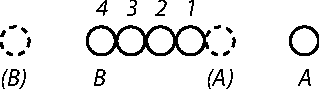
\includegraphics[width=0.36\textwidth]{gesamttex/edit_VIII,3/images/LH_35_09_23_021-022_d2.pdf}}%
  \vspace{0.5em}
  \centerline{\lbrack\textit{Fig.~2}\rbrack}%
  \label{LH_35_09_23_021v_Fig.2}%
  \vspace{1.3em}%
%  \newpage%
%
%
\pstart
\noindent causae.%
\protect\index{Sachverzeichnis}{effectus similis causae}
Nec refert
quod videntur corpora \textit{1}, \textit{2}, \textit{3} aliquam sentire debere mutationem,%
\protect\index{Sachverzeichnis}{mutatio sentita}
nam sensere utique saltem conatu,%
\protect\index{Sachverzeichnis}{conatus sentitus}
nam eo ipso dum egere passa sunt.%
\protect\index{Sachverzeichnis}{corpus agens et patiens}
\pend%
\pstart%
Si iisdem positis
corpus \textit{A} esset majus ipso \textit{B} seu \textit{4},
%
\edtext{aequale vero ipsis \textit{4.3},}{\lemma{%
aequale \lbrack...\rbrack\ \textit{4.3}}\Cfootnote{%
Die Körper \textit{4} und \textit{3} werden hierbei als eine Einheit betrachtet.}}
%
ea duo simul propellerentur%
\protect\index{Sachverzeichnis}{corpus propulsum}
et tantum \textit{1}, \textit{2} manerent intacta.%
\protect\index{Sachverzeichnis}{corpus intermedium intactum}
\pend%%
%
\pstart%
Si corpus \textit{A} esset majus quam \textit{4},
minus vero quam \textit{4.3},
nihilominus \textit{4.3}
%
\edtext{moverentur,
ipsum}{%
\lemma{moverentur,}\Bfootnote{%
\textit{(1)}~ipsam
\textit{(2)}~ipsum%
~\textit{L}}}
%
vero \textit{A} repelleretur%
\protect\index{Sachverzeichnis}{corpus repulsum}
seu eae
%
\edtext{orirentur leges%
\protect\index{Sachverzeichnis}{lex impactus}
quae essent}{%
\lemma{orirentur}\Bfootnote{%
\textit{(1)}~leges, quae minim
\textit{(2)}~leges quae essent%
~\textit{L}}}
%
si corpus \textit{A} impingeret in%
\protect\index{Sachverzeichnis}{corpus impingens}
%
\edtext{\lbrack majus\rbrack}{%
\lemma{minus}\Bfootnote{%
\textit{L~ändert Hrsg. nach ~E, S.~148}\cite{01056}}}
%
\textit{4}+\textit{3}.
\pend%%
%
\pstart%
Si corpus \textit{A} esset minus quam \textit{B},
nihilominus solum \textit{B} impelleretur%
\protect\index{Sachverzeichnis}{corpus impulsum}
intermediis intactis.%
\protect\index{Sachverzeichnis}{corpus intermedium intactum}
\pend%%
%
\pstart%
Idem est si \textit{1}, \textit{2} non essent globi similes,%
\protect\index{Sachverzeichnis}{globus}
sed alia corpora quaecunque%
\protect\index{Sachverzeichnis}{corpus quodcunque}
figurae cujuscunque.%
\protect\index{Sachverzeichnis}{figura quaecunque}
\pend%%
%
\pstart%
Eaedem conclusiones%
\protect\index{Sachverzeichnis}{conclusio probata}
aliter probari possunt
per regulas virtutis Elasticae%
\protect\index{Sachverzeichnis}{regula virtutis elasticae}%
\protect\index{Sachverzeichnis}{virtus elastica}
et flexus corporum distincte explicatos.%
\protect\index{Sachverzeichnis}{flexus corporis explicatus}
Sed tamen et hoc modo
%
\edtext{\lbrack compendiose\rbrack}{%
\lemma{compendio}\Bfootnote{%
\textit{L~ändert Hrsg.}}}
%
demonstrantur;
ut enim de jactibus aquae%
\protect\index{Sachverzeichnis}{jactus aquae}%
\lbrack:\rbrack\
quod aqua aeque alte exiliat%
\protect\index{Sachverzeichnis}{aqua exilians}
quam est altitudo columnae%
\protect\index{Sachverzeichnis}{columna aquae}%
\protect\index{Sachverzeichnis}{altitudo columnae aquae}%
\lbrack,\rbrack\
compendiose ex solo virium servatarum principio%
\protect\index{Sachverzeichnis}{principium virium servatarum}%
\protect\index{Sachverzeichnis}{vis servata}
demonstrari potest,
quod
%
\edtext{tamen et distincte}{%
\lemma{tamen}\Bfootnote{%
\textit{(1)}~distincte
\textit{(2)}~et distincte%
~\textit{L}}}
%
per pressionum gradus propagatos%
\protect\index{Sachverzeichnis}{gradus pressionis propagatus}
efficere licet;
ita et hoc loco contingit,
ut quae alia via distinctius quidem sed prolixe,
hoc loco breviter et paucis explicari possint.
%
\lbrack22~r\textsuperscript{o}\rbrack\  %  %  %  %  Blatt 22r
%
\pend%
%
\pstart%
Ex his intelligi potest,
quod natura similitudinem in omnibus servet,%
\protect\index{Sachverzeichnis}{natura servans similitudinem}%
\protect\index{Sachverzeichnis}{similitudo servata}
quando potest;
quando vero eam servare non potest
tunc contingit aequipollens.%
\protect\index{Sachverzeichnis}{aequipollens}
Ut
%
\edtext{\lbrack si\rbrack}{%
\lemma{si}\Bfootnote{%
\textit{erg. Hrsg.}}}
%
ponamus corpus \textit{A} eodem modo incurrere%
\protect\index{Sachverzeichnis}{corpus incurrens}
%
\edtext{duobus \textit{B}, \textit{C},
ipsi \textit{A} et inter se aequalibus,%
\protect\index{Sachverzeichnis}{corpora aequalia}
tunc}{%
\lemma{duobus}\Bfootnote{%
\textit{(1)}~aequalibus \textit{B}, \textit{C}, tunc
\textit{(2)}~\textit{B}, \textit{C}, % ipsi \textit{A} et inter se 
\lbrack...\rbrack\ aequalibus, tunc%
~\textit{L}}}
%
patet\lbrack:\rbrack\
cum nulla sit ratio%
\protect\index{Sachverzeichnis}{ratio praeferendi}
cur ipsum \textit{B} ipsi \textit{C} praeferatur
vel contra,
necessario utrumque percipere ictum,%
\protect\index{Sachverzeichnis}{ictus perceptus}
etiamsi inter se connexa non sint,%
\protect\index{Sachverzeichnis}{corpora connexa}
adeoque quia nulla est ratio separationis,%
\protect\index{Sachverzeichnis}{ratio separationis}%
\textls{ eodem modo moveri post ictum,
ac si fuisset corpus solidum $B+C.$}%
\protect\index{Sachverzeichnis}{corpus solidum}
Quod etiam memorabile est.
\pend%
%
%
\newpage% 
%  \vspace{1.0em}%	% Diagramm Fig.~3
  \centerline{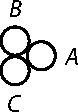
\includegraphics[width=0.086\textwidth]{gesamttex/edit_VIII,3/images/LH_35_09_23_021-022_d3.pdf}}%
  \vspace{0.5em}
  \centerline{\lbrack\textit{Fig.~3}\rbrack}%
%  \label{LH_35_09_23_022r_d2_Fig.3}%
  \vspace{1.3em}%
%  \newpage%
%
%
\pstart%
Videamus
%
\edtext{ergo,
cum}{%
\lemma{ergo,}\Bfootnote{%
\textit{(1)}~qui
\textit{(2)}~cum%
~\textit{L}}}
%
natura%
\protect\index{Sachverzeichnis}{natura}
%
\edtext{rationem%
\protect\index{Sachverzeichnis}{ratio separandi}
vel facultatem%
\protect\index{Sachverzeichnis}{facultas separandi}
(\protect\vphantom)%
id est voluntatem%
\protect\index{Sachverzeichnis}{voluntas}
vel facul\-ta\-tem%
\protect\index{Sachverzeichnis}{facultas separandi}%
\protect\vphantom()
separandi non habet,}{%
\lemma{rationem}\Bfootnote{%
\textit{(1)}~non habet
\textit{(2)}~vel facultatem \lbrack...\rbrack\ non habet,%
~\textit{L}}}
%
quomodo hanc necessariam dissimilitudinem%
\protect\index{Sachverzeichnis}{dissimilitudo causae et effectus}
inter causam et%
\protect\index{Sachverzeichnis}{causa et effectus}%
\protect\index{Sachverzeichnis}{effectus et causa}
%
\edtext{effectum aequipollentia quadam compenset.%
\protect\index{Sachverzeichnis}{aequipollentia causae et effectus}%
\protect\index{Sachverzeichnis}{aequipollentia dissimilitudinem compensans}%
}{%
\lemma{effectum}\Bfootnote{%
\textit{(1)}~compenset.
\textit{(2)}~aequipollentia quadam compenset.%
~\textit{L}}}
\pend%%
%
\pstart%
Ante omnia patet\lbrack:\rbrack\
cum corpus majus incurrit in minus quiescens,%
\protect\index{Sachverzeichnis}{corpus majus in minus quiescens}%
\protect\index{Sachverzeichnis}{corpus incurrens in minus quiescens}
tunc non posse obtineri similitudinem majori%
\protect\index{Sachverzeichnis}{corpus majus quiescens}
%
\edtext{\lbrack quiescenti\rbrack,}{%
\lemma{quiescente}\Bfootnote{%
\textit{L~ändert Hrsg.}}}
%
utique enim tunc nimium quiesceret;
multo minus poterit obtineri ipso repulso,%
\protect\index{Sachverzeichnis}{corpus majus repulsum}
ut vel hinc pateat ipsum debere progredi.%
\protect\index{Sachverzeichnis}{corpus majus progrediens}
Nam si quiescat\lbrack,\rbrack\
nimis.
Ergo concludo:
si corpus majus incurrit in minus quiescens progreditur,%
\protect\index{Sachverzeichnis}{corpus majus in minus quiescens}%
\protect\index{Sachverzeichnis}{corpus incurrens in minus quiescens}%
\protect\index{Sachverzeichnis}{corpus majus progrediens}
id enim similius statui priori,%
\protect\index{Sachverzeichnis}{status prior}
quam si quiesceret%
\protect\index{Sachverzeichnis}{corpus majus quiescens}
vel repelleretur.%
\protect\index{Sachverzeichnis}{corpus majus repulsum}
\pend%%
%
\pstart%
%
Contra:
%\edtext{}{%
%\lemma{Contra:}\Bfootnote{%
%\textit{erg.~L}}}
%
Si corpus minus incurrit in majus%
\protect\index{Sachverzeichnis}{corpus minus in majus quiescens}%
\protect\index{Sachverzeichnis}{corpus incurrens in majus quiescens}
%
\edtext{quiescens%
\lbrack,\rbrack\
repelletur,%
\protect\index{Sachverzeichnis}{corpus minus repulsum}%
}{%
\lemma{quiescens}\Bfootnote{%
\textit{(1)}~non quies
\textit{(2)}~repelletur%
~\textit{L}}}
%
neque enim progredietur,%
\protect\index{Sachverzeichnis}{corpus minus progrediens}
ita enim nimium motus erit in alteram partem;
%
\edtext{\lbrack neque\rbrack}{%
\lemma{non}\Bfootnote{\textit{L~ändert Hrsg.}}}
%
quiescet,
ita enim plus quiescet
quam ante quieverat.%
\protect\index{Sachverzeichnis}{corpus minus quiescens}
Communicabit motum suum majori,%
\protect\index{Sachverzeichnis}{motus communicatus}
sed quia ita necesse erit nimium moveri
%
\edtext{in eam}{%
\lemma{in}\Bfootnote{%
\textit{(1)}~ejus
\textit{(2)}~eam%
~\textit{L}}}
%
qua iverat plagam,%
\protect\index{Sachverzeichnis}{plaga incursus}
plus scilicet quam ante,
necesse
%
\edtext{est compensari}{%
\lemma{est}\Bfootnote{%
\textit{(1)}~id
\textit{(2)}~compensari%
~\textit{L}}}
%
hanc
ut ita loquar
injustitiam%
\protect\index{Sachverzeichnis}{compensatio injustitiae}%
\protect\index{Sachverzeichnis}{injustitia}
ipso repulso;%
\protect\index{Sachverzeichnis}{corpus repulsum}
id
%
\edtext{est
in quantum quantitas motus in plagam incursus%
\protect\index{Sachverzeichnis}{quantitas motus}%
\protect\index{Sachverzeichnis}{plaga incursus}%
\protect\index{Sachverzeichnis}{incursus corporis in majus quiescens}%
}{%
\lemma{est}\Bfootnote{%
\textit{(1)}~quanta est
\textit{(2)}~vis
\textit{(3)}~in quantum
\textit{(a)}~vis in
\textit{(b)}~quantitas motus in
\textit{(aa)}~partem in quam tendit
\textit{(bb)}~plagam incursus%
~\textit{L}}}
%
excedit quantitatem ipsius incursus,%
\protect\index{Sachverzeichnis}{quantitas incursus}%
\protect\index{Sachverzeichnis}{incursus corporis in majus quiescens}
in tantum incurrens repelletur,%
\protect\index{Sachverzeichnis}{corpus incurrens in majus quiescens}
ut scilicet in quantum similitudo servari non potest,%
\protect\index{Sachverzeichnis}{similitudo non servata}
saltem utriusque%
\lbrack,\rbrack\
plagae%
\protect\index{Sachverzeichnis}{plaga incursus}
%
\edtext{et corporis%
\protect\index{Sachverzeichnis}{corpus incurrens in majus quiescens}%
\lbrack,\rbrack%
}{%
\lemma{et}\Bfootnote{%
\hspace{-0,5mm}corporis
\textit{erg.~L}}}
%
par ratio%
\protect\index{Sachverzeichnis}{ratio par}
%
\edtext{habeatur.
Eodem}{%
\lemma{habeatur.}\Bfootnote{\hspace{-0,5mm}%
\textbar~Quod calculum
\textbar~hunc \textit{erg.}~%
\textbar\ ita dabit. \textit{gestr.}~%
\textbar\ Eodem%
~\textit{L}}}
%
modo
%
\edtext{quando majus incurrit in minus,%
\protect\index{Sachverzeichnis}{corpus majus in minus}%
\protect\index{Sachverzeichnis}{corpus incurrens in minus}}{%
\lemma{quando}\Bfootnote{%
\textit{(1)}~minus incurrit
\textit{(2)}~majus incurrit in minus,%
~\textit{L}}}
%
tunc
in quantum majus excedit minus,%
\protect\index{Sachverzeichnis}{excessus corporis majoris}
non fieret compensatio.%
\protect\index{Sachverzeichnis}{compensatio excessus}
Nimirum natura%
\protect\index{Sachverzeichnis}{natura conans ad similitudinem perfectam}
tendit efficere,
%
\edtext{ut tantum}{%
\lemma{ut}\Bfootnote{%
\textit{(1)}~corpus in
\textit{(2)}~tantum%
~\textit{L}}}
%
quiescat quantum ante quievit,
et tantum moveatur in eandem plagam%
\protect\index{Sachverzeichnis}{plaga incursus}
quantum ante motum est;
sed quia id efficere non potest
sine penetratione dimensionum%
\protect\index{Sachverzeichnis}{penetratio dimensionum}
aut divulsione corporum,%
\protect\index{Sachverzeichnis}{divulsio corporis}
%
\edtext{\lbrack quarum neutra\rbrack}{%
\lemma{quorum neutrum}\Bfootnote{%
\textit{L~ändert Hrsg.}}}
%
hic fieri posse supponitur,
ideo quam proxime licet
id assequi conabitur.
\edlabel{LH_35_09_23_022r_tejx-1}%
Primum ergo,
in quantum corpus majus incurrens in minus%
\protect\index{Sachverzeichnis}{corpus majus in minus}%
\protect\index{Sachverzeichnis}{corpus incurrens in minus}
partem habet minori aequalem,
in tantum minori
%
\edtext{dabit}{%
\lemma{dabit}\Bfootnote{%
\textit{erg.~L}}}
%
suam celeritatem,%
\protect\index{Sachverzeichnis}{celeritas corpori minori data}
et pars illa
%
\edtext{quiescere deberet,
pars}{%
\lemma{quiescere}\Bfootnote{%
\textit{(1)}~debet
\textit{(2)}~deberet
\textit{(a)}~. Sed
\textit{(b)}~, pars%
~\textit{L}}}
%
\edtext{autem majoris residua}{%
\lemma{autem}\Bfootnote{%
\textit{(1)}~residua
\textit{(2)}~majoris residua%
~\textit{L}}}
%
deberet procedere cum
%
\edtext{corpore excipiente}{%
\lemma{corpore}\Bfootnote{%
\hspace{-0,5mm}excipiente
\textit{erg.~L}}}
%
minore,%
\protect\index{Sachverzeichnis}{corpus excipiens minus}
retenta
%
\edtext{celeritate.%
\protect\index{Sachverzeichnis}{celeritas corporis majoris retenta}
Atque}{%
\lemma{celeritate}\Bfootnote{\hspace{-0,5mm}%
\textbar~, sed quia ea non potest procedere quin secum abripiat eam quae quiescere deberet minori aequalem, ideo eam quidem secum abripit, sed tanto tardius \textit{gestr.}~%
\textbar~. Atque%
~\textit{L}}}
%
ita haberetur perfecta%
\protect\index{Sachverzeichnis}{similitudo status prioris perfecta}
%
\edtext{similitudo status}{%
\lemma{similitudo}\Bfootnote{\hspace{-0,5mm}%
\textbar~esse \textit{gestr.}~%
\textbar\ status%
~\textit{L}}}
%
provenientis et%
\protect\index{Sachverzeichnis}{status proveniens}
%
\edtext{prioris.%
\protect\index{Sachverzeichnis}{status prior}
Et cum natura%
\protect\index{Sachverzeichnis}{natura conans ad similitudinem perfectam}%
}{%
\lemma{prioris.}\Bfootnote{%
\textit{(1)}~Verum quia pars
\textit{(2)}~Et cum natura%
~\textit{L}}}
%
conetur ad perfectam hanc%
\protect\index{Sachverzeichnis}{conatus naturae ad similitudinem perfectam}
%
\edtext{similitudinem,%
\protect\index{Sachverzeichnis}{similitudo status prioris perfecta}
hinc}{%
\lemma{similitudinem,}\Bfootnote{%
\textit{(1)}~utique
\textit{(2)}~hinc%
~\textit{L}}}
%
erit
%
\edtext{in minori seu excipiente%
\protect\index{Sachverzeichnis}{corpus excipiens minus}
conatus}{%
\lemma{in}\Bfootnote{%
\textit{(1)}~minori con
\textit{(2)}~minori seu excipiente conatus%
~\textit{L}}}
%
progrediendi%
\protect\index{Sachverzeichnis}{conatus progrediendi}
celeritate majoris incurrentis.%
\protect\index{Sachverzeichnis}{celeritas corporis majoris}%
\protect\index{Sachverzeichnis}{celeritas corporis incurrentis}
In parte majoris
quae minori aequalis est
erit quies,%
\protect\index{Sachverzeichnis}{quies corporis incurrentis}
in reliqua parte erit conatus se ab hac separandi%
\protect\index{Sachverzeichnis}{conatus separandi}
seu ultra
%
\edtext{progrediendi%
\protect\index{Sachverzeichnis}{conatus progrediendi}
priori celeritate,
id est excessus conabitur%
\protect\index{Sachverzeichnis}{conatus excessus}
abire cum minori;
quod cum ob cohaesionem corporum%
\protect\index{Sachverzeichnis}{cohaesio corporis}
fieri nequeat,}{%
\lemma{progrediendi,}\Bfootnote{%
\textit{(1)}~quod cum fieri nequeat,
\textit{(2)}~priori celeritate, % id est excessus conabitur abire cum minori; quod cum 
\lbrack...\rbrack\ ob cohaesionem
\textit{(a)}~corporis
\textit{(b)}~corporum fieri nequeat,%
~\textit{L}}}
%
necesse erit
ut pars illa
quae pergere conatur,
secum abripiat quiescentem,%
\protect\index{Sachverzeichnis}{abreptio quiescentis}
sed tanto tardius,
in ea scilicet ratione
quae est excessus%
\protect\index{Sachverzeichnis}{excessus celeritatis}
ad corpus totum,%
\protect\index{Sachverzeichnis}{corpus excipiens minus}
et ita prodit plane nostrum
%
\edtext{theorema superius.%
\edlabel{LH_35_09_23_022r_tejx-2}%
}{%
\lemma{theorema%
\protect\index{Sachverzeichnis}{theorema}
superius}\Cfootnote{%
N.~\ref{dcc_01}, %??S01\textsubscript{1}
S.~\refpassage{LH_35_09_23_002r_majausinminus_bfnd-1}{LH_35_09_23_002r_majausinminus_bfnd-2},
\refpassage{LH_35_09_23_002v_majusinminquiesc_jksr-3}{LH_35_09_23_002v_majusinminquiesc_jksr-2};
N.~\ref{dcc_02-1}, %??S01\textsubscript{2}
S.~\refpassage{LH_35_09_23_003v_kregs-1}{LH_35_09_23_003v_kregs-2}.}}
%
\edtext{Sed videndum}{%
\lemma{Sed}\Bfootnote{%
\textit{(1)}~ostendendum
\textit{(2)}~videndum%
~\textit{L}}}
%
est tamen paulo distinctius,
an hoc modo obtineatur maxima similitudo possibilis.%
\protect\index{Sachverzeichnis}{similitudo maxima}
Inquirendum est autem
tum in quo consistat hoc loco similitudo
seu ad eam appropinquatio;%
\protect\index{Sachverzeichnis}{appropinquatio ad similitudinem}
tum
%
\edtext{\lbrack an\rbrack}{%
\lemma{quod}\Bfootnote{%
\textit{L~ändert Hrsg.}}}
%
sic obtineatur maxima similitudo possibilis.%
\protect\index{Sachverzeichnis}{similitudo maxima}
\pend%
%\newpage%
%
\pstart%
Circa similitudinem statuum%
\protect\index{Sachverzeichnis}{similitudo statuum}
sequentia notanda,
status quietis%
\protect\index{Sachverzeichnis}{status quietis}%
\protect\index{Sachverzeichnis}{quies corporis incurrentis}
similior est regressui%
\protect\index{Sachverzeichnis}{regressus corporis incurrentis}
vel progressui,%
\protect\index{Sachverzeichnis}{progressus corporis incurrentis}
quam regressus vel progressus sibi invicem.
Quies similior est\lbrack,\rbrack\
%
\edtext{seu natura propior,%
\protect\index{Sachverzeichnis}{similior seu natura propior}
minori progressui vel minori regressui;
quam \lbrack majori\rbrack.
Item progressus vicinior minori regressui
quam majori,
et contra.}{%
\lemma{seu}\Bfootnote{%
\textit{(1)}~vi
\textit{(2)}~natura propior,
\textit{(a)}~major
\textit{(b)}~minori progressui vel
\textit{(aa)}~regressui quam
\textit{(bb)}~majori
\textit{(cc)}~minori regressui; quam
\textbar~minori \textit{ändert Hrsg. nach~E, S.~150\cite{01056}}~%
\textbar~. Item
\textit{(aaa)}~vic
\textit{(bbb)}~progressus vicinior
\textit{(aaaa)}~majori
\textit{(bbbb)}~minori regressui % quam majori, 
\lbrack...\rbrack\ et contra.%
~\textit{L}}}
%
\lbrack22~v\textsuperscript{o}\rbrack\  %  %  %  %  Blatt 22v
%
Item quies%
\protect\index{Sachverzeichnis}{quies corporis incurrentis}
similior est minori progressui,
quam majori regressui
et contra minori regressui%
\protect\index{Sachverzeichnis}{progressus corporis incurrentis}
quam majori
\edlabel{LH_35_09_23_022v_wedl-1}%
progressui.%
\protect\index{Sachverzeichnis}{progressus corporis incurrentis}
%
\edtext{}{%
{\xxref{LH_35_09_23_022v_wedl-1}{LH_35_09_23_022v_wedl-2}}%
{\lemma{progressui}\Bfootnote{%
\textit{(1)}~Repulsa
\textit{(2)}~Repelli corpus
\textit{(3)}~\textbar~Aliqua \textit{erg.}~%
\textbar\ Repulsa corporis
\textit{(a)}~majoris
\textit{(b)}~minoris
\textit{(c)}~minoris in % motu existentis vicinior 
\lbrack...\rbrack\ est quieti
\textit{(aa)}~minoris
\textit{(bb)}~majoris
\textbar~%
\textit{(1)}~ejusdem in motu
\textit{(2)}~in eodem motu existentis \textit{erg.}~%
\textbar~, quam quies 
\textit{(aaa)}~majoris
\textit{(bbb)}~minoris
\textit{(ccc)}~ejusdem minoris.%
~\textit{L}}}}
%
\pend%%
%
\pstart%
Aliqua Repulsa corporis minoris%
\protect\index{Sachverzeichnis}{repulsa corporis minoris}
in motu existentis
vicinior est quieti majoris%
\protect\index{Sachverzeichnis}{quies corporis majoris}
in eodem motu existentis,
quam quies ejusdem minoris.%
\edlabel{LH_35_09_23_022v_wedl-2}
%
Nam in
%
\edtext{quiete minoris,%
\protect\index{Sachverzeichnis}{quies corporis minoris}%
}{%
\lemma{quiete}\Bfootnote{%
\textit{(1)}~majoris
\textit{(2)}~minoris%
~\textit{L}}}
%
exprimitur quies partis
%
\edtext{majoris minori aequalis.
Sed quies}{%
\lemma{majoris}\Bfootnote{%
\textit{(1)}~, sed pars
\textit{(2)}~minori aequalis. Sed quies%
~\textit{L}}}
%
excessus%
\protect\index{Sachverzeichnis}{excessus celeritatis}
nullo modo exprimitur vel compensatur.
%
\edtext{Itaque
ubi corpus aliquod majus sisteretur,%
\protect\index{Sachverzeichnis}{corpus majus sistens}%
}{%
\lemma{Itaque}\Bfootnote{%
\textit{(1)}~non sisti tan
\textit{(2)}~cum corpus aliquod
\textit{(3)}~ubi corpus aliquod majus sisteretur,%
~\textit{L}}}
%
ibi corpus minus debet plus quam sisti,
id est repelli.%
\protect\index{Sachverzeichnis}{corpus minus repulsum}
Est enim repulsa%
\protect\index{Sachverzeichnis}{repulsa corporis incurrentis}
plus quam quies%
\protect\index{Sachverzeichnis}{quies corporis incurrentis}
seu repelli plus quam sisti.%
\protect\index{Sachverzeichnis}{repelli plus quam sisti}
%
\edtext{Ergo ubi corpus majus quiesceret,%
\protect\index{Sachverzeichnis}{corpus majus quiescens}%
}{%
\lemma{Ergo}\Bfootnote{%
\textit{(1)}~quies
\textit{(2)}~ubi corpus majus quiesceret,%
~\textit{L}}}
%
ibi debet minus plus quam quiescere,
compensationis causa,%
\protect\index{Sachverzeichnis}{compensatio excessus}
id est
\edlabel{LH_35_09_23_022v_mshx-1}%
repelli.%
\protect\index{Sachverzeichnis}{corpus minus repulsum}
%
\edtext{}{%
{\xxref{LH_35_09_23_022v_mshx-1}{LH_35_09_23_022v_mshx-2}}%
{\lemma{repelli.}\Bfootnote{%
\textit{(1)}~Tamen alia repulsa
\textit{(2)}~Est
\textit{(3)}~Potest tamen ea repulsa esse%
~\textit{L}}}}
%
\pend%
%
\pstart%
Potest tamen ea repulsa%
\protect\index{Sachverzeichnis}{repulsa corporis incurrentis}
esse%
\edlabel{LH_35_09_23_022v_mshx-2}
nimia,
%
id est potest esse talis,
ut minor aliqua sit vicinior,
quaeritur ergo minima apta,%
\protect\index{Sachverzeichnis}{repulsa minima}
seu vicinissima.
\pend%%
%
\pstart%

%
\edtext{Aliqua}{%
\lemma{Aliqua}\Bfootnote{%
\textit{erg.~L}}}
%
Progressio%
\protect\index{Sachverzeichnis}{progressio corporis majoris}
%
\edtext{majoris in motu existentis vicinior est}{%
\lemma{majoris}\Bfootnote{%
\textit{(1)}~est
\textit{(2)}~\textbar~in motu existentis
\textit{erg.}~\textbar\ vicinior est%
~\textit{L}}}
%
quieti minoris%
\protect\index{Sachverzeichnis}{quies corporis minoris}
%
\edtext{in eodem motu existentis,}{%
\lemma{in}\Bfootnote{%
\hspace{-0,5mm}eodem motu existentis
\textit{erg.~L}}}
%
quam quies majoris.%
\protect\index{Sachverzeichnis}{quies corporis majoris}
Nam si
%
\edtext{minus in motu existens debet quiescere,}{%
\lemma{minus}\Bfootnote{%
\textit{(1)}~debet quies
\textit{(2)}~in motu existens debet quiescere,%
~\textit{L}}}
%
debebit majus in motu existens minus quam quiescere,
id est magis a quiete recedere sive progredi.
Quia
%
\edtext{scilicet natura corpori accomodat celeritatem;%
\protect\index{Sachverzeichnis}{natura celeritatem corpori accomodans}
sive si natura parvitatem corporis
quod quiescere debet
assequi non potest,}{%
\lemma{scilicet}\Bfootnote{%
\hspace{-0,5mm}natura
\textit{(1)}~defectum
\textit{(2)}~exces
\textit{(3)}~corpori
\textit{(a)}~magnitudinem
\textit{(b)}~accomodat celeritatem; sive
\textit{(aa)}~si
\textit{(aaa)}~magnitudine corporis quietem assequi
\textit{(bbb)}~quietis
\textit{(bb)}~\textbar~si natura \textit{erg.}~%
\textbar\ parvitatem corporis quod quiescere debet
\textbar~si natura \textit{erg. u. gestr.}~%
\textbar\ assequi non potest,%
~\textit{L}}}
%
seu si id quod quiescere deberet
%
\edtext{esset nimis magnum,}{%
\lemma{esset}\Bfootnote{%
\textit{(1)}~minus
\textit{(2)}~nimis magnum,%
~\textit{L}}}
%
\edtext{tunc aliquid}{%
\lemma{tunc}\Bfootnote{%
\textit{(1)}~quod
\textit{(2)}~aliquid%
~\textit{L}}}
%
motus ei adjicit.
Quaerenda paulo aptior enuntiatio:%
\protect\index{Sachverzeichnis}{enuntiatio aptior}
Si majus justo quiesceret,
tunc nimium quiesceretur,
ergo corpus minus sisti,
majus progredi compensationem habent.%
\protect\index{Sachverzeichnis}{compensatio excessus}
\pend%%
%
\pstart%
Quando corpus \textit{A}
%
\edtext{majus}{%
\lemma{majus}\Bfootnote{%
\textit{erg.~L}}}
%
incurrit in corpus \textit{B} minus,%
\protect\index{Sachverzeichnis}{corpus majus in minus}%
\protect\index{Sachverzeichnis}{corpus incurrens in minus}
tunc,
si excessus est infinite%
\protect\index{Sachverzeichnis}{excessus infinite parvus}
%
\edtext{parvus,
progredietur}{%
\lemma{parvus,}\Bfootnote{%
\textit{(1)}~quies
\textit{(2)}~progredietur%
~\textit{L}}}
%
corpus \textit{A}%
\protect\index{Sachverzeichnis}{progressus corporis incurrentis}
celeritate etiam infinite parva;%
\protect\index{Sachverzeichnis}{celeritas infinite parva}
si vero major,
etiam majore aliqua celeritate progredietur.%
\protect\index{Sachverzeichnis}{celeritas corporis incurrentis post incursum}
Quaeritur autem
an ea sic
(\protect\vphantom)%
ut
\edtext{paulo ante}{%
\lemma{paulo ante}\Cfootnote{%
S.~\refpassage{LH_35_09_23_022r_tejx-1}{LH_35_09_23_022r_tejx-2}.%
}}
dixi%
\protect\vphantom()
determinanda sit,
ut corpus quidem excipiens%
\protect\index{Sachverzeichnis}{corpus excipiens minus}
primum a parte majoris incurrentis%
\protect\index{Sachverzeichnis}{corpus incurrens majus}
sibi aequali
accipiat celeritatem ejus
(id est celeritatem incursus)%
\protect\index{Sachverzeichnis}{celeritas incursus}
parte illa majoris vicissim quiescente;
altera vero pars
%
\edtext{majoris seu excessus
cum excipiente etiam
celeritate incursus%
\protect\index{Sachverzeichnis}{celeritas incursus}
procedere conetur,}{%
\lemma{majoris}\Bfootnote{%
\textit{(1)}~procedat
\textit{(2)}~seu excessus \lbrack...\rbrack\ procedere conetur,%
~\textit{L}}}
%
sed cum id
nisi quiescente simul abrepto%
\protect\index{Sachverzeichnis}{corpus quiescens abreptum}
nequeat,
eo ipso gravabitur seu eatenus tardius procedet.
Quaeritur inquam
an ad quaesitum effectum%
\protect\index{Sachverzeichnis}{effectus quaesitus}
nulla ratione accedi possit propius.
Quaesitus effectus erat ut solum
%
\edtext{excipiens aut ipsi aequale quiesceret,}{%
\lemma{excipiens}\Bfootnote{%
\textit{(1)}~quiesceret
\textit{(2)}~aut ipsi aequale quiesceret,%
~\textit{L}}}
%
majus aut ipsi aequipollens%
\protect\index{Sachverzeichnis}{corpus aequipollens}
%
\edtext{progrederetur.
Patet ante omnia
non posse excipiens progredi tardius
quam celeritate}{%
\lemma{progrederetur.}\Bfootnote{%
\textit{(1)}~Hoc loco excipiens pro
\textit{(2)}~Patet ante % omnia non posse excipiens progredi 
\lbrack...\rbrack\ tardius quam
\textit{(a)}~ratione
\textit{(b)}~celeritate%
~\textit{L}}}
%
quam assignavi,
ergo
%
\edtext{si mutatione aliqua facta%
\protect\index{Sachverzeichnis}{mutatio fata}
propius}{%
\lemma{si}\Bfootnote{%
\textit{(1)}~propius
\textit{(2)}~mutatione aliqua facta propius%
~\textit{L}}}
%
accedendum esset ad effectum desideratum,%
\protect\index{Sachverzeichnis}{effectus desideratus}
deberet fingi corpus excipiens moveri
%
\edtext{celerius,
quoniam enim}{%
\lemma{celerius,}\Bfootnote{%
\textit{(1)}~nam quia
\textit{(2)}~quoniam enim%
~\textit{L}}}
%
id quod moveri debet,
debet esse aequale impingenti majori,%
\protect\index{Sachverzeichnis}{corpus impingens majus}
et quod quiescere excipienti minori,%
\protect\index{Sachverzeichnis}{corpus excipiens minus}
ideo possemus excipiens\lbrack,\rbrack\
licet minus\lbrack,\rbrack\
movere tanto majori celeritate ad compensandum,
et ita incurrens
%
\edtext{quiesceret.
Sed hoc quidem parum consentaneum rationi.%
\protect\index{Sachverzeichnis}{consentaneum rationi}
Vel denique quaerendum erit medium}{%
\lemma{quiesceret.}\Bfootnote{%
\textit{(1)}~Vel denique dabitur me
\textit{(2)}~Sed hoc \lbrack...\rbrack\ erit medium%
~\textit{L}}}
%
ut accessio%
\protect\index{Sachverzeichnis}{accessio effectus causae}
seu assimilatio%
\protect\index{Sachverzeichnis}{assimilatio effectus causae}
tam quaeratur in excipiente
quam in incurrente.
Si quaeratur in excipiente solo,%
\protect\index{Sachverzeichnis}{corpus excipiens minus}
tota
ut dixi
virtus ei tribuetur,%
\protect\index{Sachverzeichnis}{virtus tributa excipienti}
seu omnino auferetur ab incurrente;%
\protect\index{Sachverzeichnis}{virtus ab incurrente ablata}
si quaeratur remedium%
\protect\index{Sachverzeichnis}{remedium}
in incurrente solo,%
\protect\index{Sachverzeichnis}{corpus incurrens majus}
habebitur impossibile,
id est penetratio dimensionum;%
\protect\index{Sachverzeichnis}{penetratio dimensionum}
via ergo a nobis electa quaeretur in
%
\edtext{utroque.
Illud vero observatur,}{%
\lemma{utroque}\Bfootnote{%
\textit{(1)}~, et utrumque corpus
\textit{(2)}~. Illud vero observatur,%
~\textit{L}}}
%
quod rationi consentaneum est,%
\protect\index{Sachverzeichnis}{consentaneum rationi}
ut corpori incurrenti%
\protect\index{Sachverzeichnis}{corpus incurrens majus}
quam minimum auferatur sua vis,%
\protect\index{Sachverzeichnis}{vis ablata ab incurrente}
nec in quantum necesse est,
nec tamen in totum relinquatur,
quia si minus esset paulo\lbrack,\rbrack\
plane
%
quiesceret,
\textlangle nunc\textrangle\ ergo
%\edtext{}{%
%\lemma{quiesceret,}\Bfootnote{%
%\textit{(1)}~\textlangle tunc\textrangle
%\textit{(2)}~ergo%
%~\textit{L}}}
%
progredietur equidem eo
%
\edtext{quo explicui modo,%
\protect\index{Sachverzeichnis}{modus progrediendi}%
}{%
\lemma{quo explicui modo}\Cfootnote{%
ebd.}}
%
sed tardius tamen
quam si nihil occurrisset.
\pend%%
%
\pstart%
Quando corpus \textit{A} incurrit in corpus \textit{B} majus,%
\protect\index{Sachverzeichnis}{corpus minus in majus}%
\protect\index{Sachverzeichnis}{corpus incurrens in majus}
tunc primum
in quantum majus partem habet minori aequalem,
in
%
\edtext{tantum motum recipit,
et minus incurrens quiescit.}{%
\lemma{tantum}\Bfootnote{%
\textit{(1)}~quie
\textit{(2)}~motum recipit
\textit{(a)}~minus
\textit{(b)}~, et
\textit{(aa)}~quiescit
\textit{(bb)}~minus incurrens quiescit.%
~\textit{L}}}
%
Sed quia majus indissolubile est,%
\protect\index{Sachverzeichnis}{corpus indissolubile}
ideo non potest pars moveri quin altera pars
%
\edtext{moveatur.
Sed}{%
\lemma{moveatur.}\Bfootnote{%
\textit{(1)}~Nec tame
\textit{(2)}~Sed%
~\textit{L}}}
%
hoc modo minus quiesceret,
majus vero totum motum reciperet,
quod est absurdum,%
\protect\index{Sachverzeichnis}{absurdum}
et valde
%
\edtext{dissimile,
et maxime apparet dissimilitudo,%
\protect\index{Sachverzeichnis}{dissimilitudo maxima}%
}{%
\lemma{dissimile}\Bfootnote{\hspace{-0,5mm}%
\textit{(1)}~a praesenti inprimis
\textit{(2)}~, et maxime apparet dissimilitudo,%
~\textit{L}}}
%
quando excipiens est valde magnum,%
\protect\index{Sachverzeichnis}{corpus excipiens valde magnum}
itaque
%
\edtext{dividi necesse est}{%
\lemma{dividi}\Bfootnote{%
\textit{(1)}~potest
\textit{(2)}~necesse est%
~\textit{L}}}
%
mutationem inter corpora,%
\protect\index{Sachverzeichnis}{mutatio divisa inter corpora}
et incurrens nonnihil repelletur.%
\protect\index{Sachverzeichnis}{corpus incurrens repulsum}
\pend%
%
\pstart%
Omnia haec explicanda accuratius,
tum et quaenam sit ex his principiis%
\protect\index{Sachverzeichnis}{principium}
vis percus\-sio\-nis.%
\protect\index{Sachverzeichnis}{vis percussionis}
\pend%
\count\Bfootins=1000%
\count\Afootins=1200%
\count\Cfootins=1000
%
%
%    %    %    %    Ende des Textes auf Blatt 22v
%
%